
%
%
% SRP
%
%
    
\subsection{Princípio da Responsabilidade Única (Single Responsibility Principle - SRP)}
    
    \par O SRP preconiza que um módulo, ou mais comumente uma classe, deve ter uma, e apenas uma, razão para mudar, o que implica ser responsável por um único ator ou aspecto da funcionalidade do sistema. Este princípio está intimamente ligado ao conceito de coesão, onde um módulo coeso agrupa funcionalidades que servem a um único propósito bem definido. O objetivo é garantir que cada classe realize uma tarefa específica, simplificando sua compreensão e manutenção \cite{livro:martin:cleanarch}.

    \par A aplicação do SRP é vital, pois assegura que cada classe permaneça dedicada a uma tarefa específica, o que, por sua vez, simplifica seu entendimento, manutenção e potencial de expansão. Quando as classes seguem o SRP, elas se tornam mais diretas para refatorar, testar e estender, e modificações são menos propensas a afetar outras partes do sistema, minimizando o risco de introduzir erros. Isso é um contraste com classes que acumulam múltiplas responsabilidades, as quais se tornam complexas e frágeis \cite{artigo:ramachandrappa:2024}.

    \par O exemplo de violação do SRP, pode ser visualizado na Figura~\ref{fig:figura_srp_bad} que mostra a organização de uma classe antes da aplicação do princípio.

    \begin{figure}[H]
        \centering
        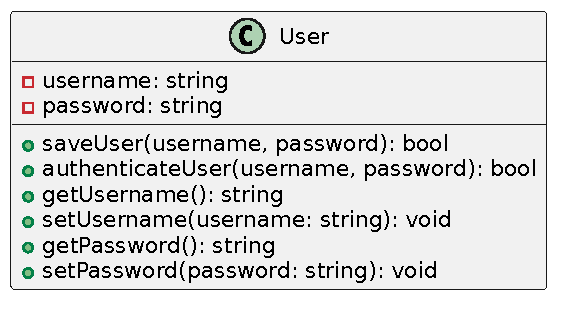
\includegraphics[width=0.8\linewidth]{figuras/solid/srp_bad.pdf}
        \caption{Violação do SRP.} 
        \label{fig:figura_srp_bad} 
        \newcommand{\minhafonte}{Fonte: Adaptado de \cite{artigo:ramachandrappa:2024}.}
        \minhafonte
    \end{figure}

    \par Nesse exemplo trazido por \cite{artigo:ramachandrappa:2024} a classe User lida tanto com a gestão dos dados do usuário (como nome e senha) quanto com a lógica de autenticação desse usuário no método authenticateUser(). A Figura~\ref{fig:figura_srp_good} ilustra a classe após a refatoração para fazer uso do SRP.

   \begin{figure}[H]
        \centering
        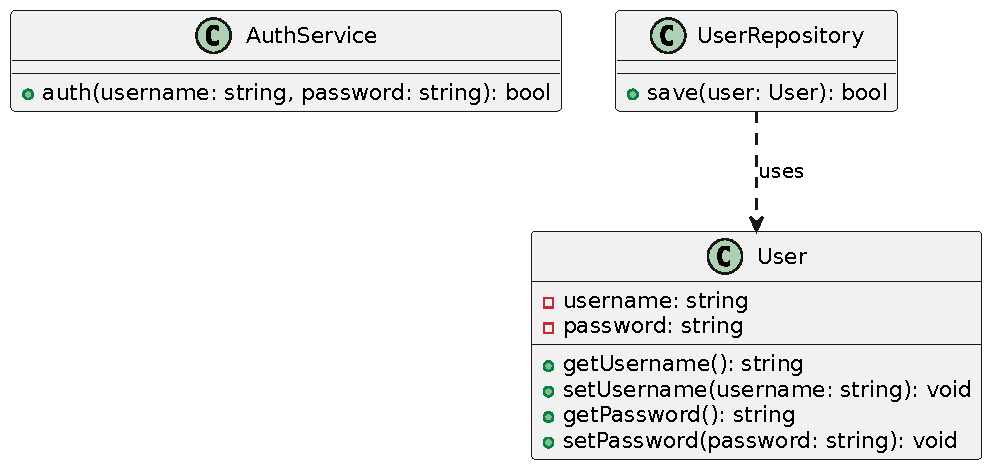
\includegraphics[width=1\linewidth]{figuras/solid/srp_good.pdf}
        \caption{Aplicação do SRP.}
        \label{fig:figura_srp_good} 
        \newcommand{\minhafonte}{Fonte: Adaptado de \cite{artigo:ramachandrappa:2024}.}
        \minhafonte
    \end{figure}

    \par Na Figura~\ref{fig:figura_srp_good} a classe User mantêm apenas os dados, a classe UserRepository controla a persistência e AuthService gerenciaria a autenticação, assim demonstrando o uso da SRP, onde cada classe tem sua própria responsabilidade \cite{artigo:ramachandrappa:2024}.

        